\documentclass[margin=5mm]{standalone}
\usepackage{tikz}
\definecolor{capri}{rgb}{0.0, 0.75, 1.0}
\begin{document}

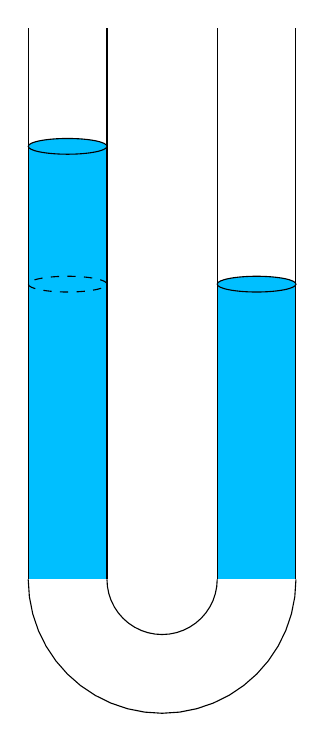
\begin{tikzpicture}
  %Inner Radius
  \pgfmathsetmacro{\rI}{0.7}

  %Height
  \pgfmathsetmacro{\h}{7}

  %Diameter of the pipe
  \pgfmathsetmacro{\d}{1}

  %Outer Radius
  \pgfmathsetmacro{\rO}{\rI + \d}

  \pgfmathsetmacro{\s}{2}

  %%Inner Part
  \draw (0,0) -- (0,-\h) coordinate (I1); 
  \draw[shift=(I1),xshift=\rI cm] plot[domain=270:90] ({\rI*sin(\x)},{\rI*cos(\x)}) coordinate (I2);
  \draw (I2) -- ++(0,\h);

  %% Outer Part
  \draw (-\d,0) -- ++(0,-\h) coordinate (O1);
  \draw[shift=(O1),xshift=\rO cm] plot[domain=270:90] ({\rO*sin(\x)},{\rO*cos(\x)}) coordinate (O2);
  \draw (O2) -- ++(0,\h);

  % NEW
  \draw[capri, line width=28pt] (-\d/2.0,-0.5*\h+\s) -- ++(0,-0.5*\h-\s) coordinate (L1);
  \draw[fill=capri] (-\d/2.0, -0.5*\h+\s) ellipse (0.5 and 0.1);
  \draw[dashed] (-\d/2.0, -0.75*\h+\s) ellipse (0.5 and 0.1);

  \draw[capri, line width=28pt] (3.8/\d/2.0, -0.75*\h+\s) -- ++(0,-0.25*\h-\s) coordinate (L2);
  \draw[fill=capri] (3.8*\d/2.0, -0.75*\h+\s) ellipse (0.5 and 0.1);

  %% l Line
%   \draw (-\d/2.0,-0.5*\h+\s) -- ++(0,-0.5*\h-\s) coordinate (L1);
%   \pgfmathsetmacro{\rl}{\rO - 0.5*\d}
%   \draw[shift=(L1),xshift=\rl cm] plot[domain=270:90] ({\rl*sin(\x)},{\rl*cos(\x)}) node[below=1.2cm,pos=0.5]{$l$} coordinate (L2);
%   \draw (L2) -- ++(0,0.5*\h-\s);

%   \draw[->] (-3,-\h-\rO) -- (-3,0) node[left]{\small Ort $y$};
%   \draw (-3.1,-0.5*\h) node[left]{$0$} -- ++(0.2,0);
\end{tikzpicture}

\end{document}